\section{Konzept 4}
Konzept vier verwendet als Partikelquelle Kerzen als Rauchentwickler. Weiterhin basiert die Funktionsweise der Konzepte nicht auf Ventilen als Schaltvorrichtungen sondern auf Schiebern oder Drehscheiben, die die Leitungssysteme translatorisch oder rotatorisch umleiten k\"{o}nnen. Hierbei m\"{u}ssen die Schaltvorrichtungen eventuell mit konstruiert werden, da sie nicht unbedingt im Handel erh\"{a}ltlich sind.

\subsection{Aufbau}
Die Versuchseinrichtung besteht aus mehreren Kerzen, einem Verd\"{u}nner und einem Thermokonditionierer, einer Schaltvorrichtung, einem Ventilator und dem zu testenden Messger\"{a}t. Zur Schaltvorrichtung f\"{u}hrt eine Leitung von den Kerzen und eine Leitung aus der Umgebungsluft. Ein Auslasskanal befindet sich in der Schaltvorrichtung, an dem sich weiterhin ein extern angeschlossener Ventilator befindet. Zwischen der Schaltvorrichtung und den Kerzen sind der Verd\"{u}nner und der Thermokonditionierer geschaltet. Die Verbindung zum Messger\"{a}t ist abschlie{\ss}end mit einem Adapterrohr gel\"{o}st. F\"{u}r die Leitungen im System ist hier noch nicht endg\"{u}ltig beschlossen, ob es sich um Rohre oder Schl\"{a}uche handeln wird. Ausschlaggebend wird hier die Schaltvorrichtung sein, da Drehscheiben mit Schl\"{a}uchen arbeiten und Schieber mit Rohren.
\begin{figure}[H]
        \myfloatalign
        \subfloat[Schieberschaltvorrichtung Stellung 0]
        {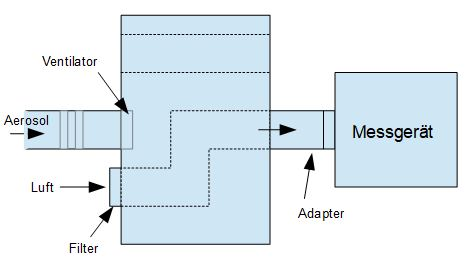
\includegraphics[width=.45\linewidth]{gfx/concepts/Konzept_4_Schieber_Zu.jpg}} \quad
        \subfloat[Rotationschaltvorrichtung Stellung 0]
        {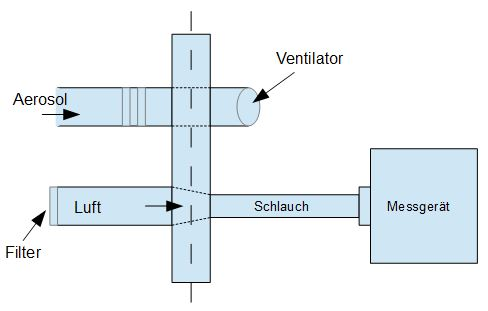
\includegraphics[width=.45\linewidth]{gfx/concepts/Konzept_4_Dreh_Zu.jpg}} 
        \caption[Geschlossene Stellung bei Schieber und Drehscheibe]
        {Geschlossene Stellung bei Schieber und Drehscheibe}
        \label{fig:concepts_4_off}
\end{figure}

\subsection{Funktionsweise}
Das Messger\"{a}t saugt in der ersten Phase der Messung, der Nullphase, Umgebungsluft an, welche \"{u}ber einen Filter gereinigt wird. Die Schaltvorrichtung befindet sich hierbei in \textit{Stellung 0}, um den Aerosoleinlass zu schlie{\ss}en. Dieser Mechanismus dient zur \"{U}berbr\"{u}ckung der Totzeit des Messger\"{a}tes, welche zwischen den Ger\"{a}ten variiert. W\"{a}hrend dieser Nullphase saugt der extern angeschlossene Ventilator den Aerosolstrom an, welcher in die Umgebungsluft entweicht. So wird der Partikelstrom bereits aufgebaut und weitere Totzeit des Systems \"{u}berwunden. Die Partikel passieren dabei den Verd\"{u}nner um die zu hohe Partikelanzahlkonzentration f\"{u}r die Messger\"{a}te zu regulieren.  Der Verd\"{u}nner scheidet jedoch einen zu geringen Volumenstrom aus, weshalb der Thermokondionierer zugeschaltet wird. Dieser erh\"{o}ht den abgegebenen Volumenstrom des Verd\"{u}nners und reguliert zus\"{a}tzlich die Temperatur des Tr\"{a}gergases\cite{candle}.\\
Nach Ablauf einer fest eingestellten Zeit schaltet das System die Leitungen um und leitet den aufgebauten Aerosolstrom in das Messger\"{a}t. Die Frischluftzufuhr ist in dieser \textit{Stellung 1} gestoppt und der Partikelsprung findet statt. Die Schaltvorg\"{a}nge werden beliebig oft wiederholt. Der Wechsel zwischen Frischluft und Aerosolstrom verst\"{a}rkt das generierte Sprungsignal am Messger\"{a}t.\\
Um die Totzeit des Systems so gering wie m\"{o}glich zu halten, werden die Leitung in der Schaltvorrichtung und die Leitung zum Messger\"{a}t so kurz wie m\"{o}glich gehalten. Die Gesamttotzeit ergibt sich so aus der Totzeit des Messger\"{a}tes und der Schaltzeit der Schaltvorrichtung.
\begin{figure}[H]
        \myfloatalign
        \subfloat[Schieberschaltvorrichtung Stellung 1]
        {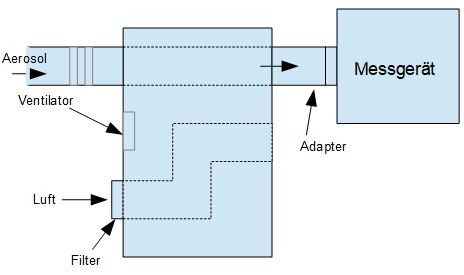
\includegraphics[width=.45\linewidth]{gfx/concepts/Konzept_4_Schieber_Auf.jpg}} \quad
        \subfloat[Rotationschaltvorrichtung Stellung 1]
        {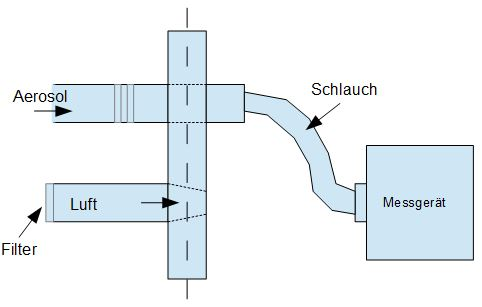
\includegraphics[width=.45\linewidth]{gfx/concepts/Konzept_4_Dreh_Auf.jpg}} 
        \caption[Offene Stellung bei Schieber und Drehscheibe]
        {Offene Stellung bei Schieber und Drehscheibe}
        \label{fig:concepts_4_on}
\end{figure}